\documentclass[11pt]{article}

\newcommand{\cnum}{CM146}
\newcommand{\ced}{Winter 2018}
\newcommand{\ctitle}[3]{\title{\vspace{-0.5in}\cnum, \ced\\Problem Set #1: #2}}

\newcommand{\solution}[1]{{{\color{blue}{\bf Solution:} {#1}}}}
\usepackage[usenames,dvipsnames,svgnames,table,hyperref]{xcolor}
\usepackage{graphicx}

\graphicspath{{images/}}

\renewcommand*{\theenumi}{\alph{enumi}}
\renewcommand*\labelenumi{(\theenumi)}
\renewcommand*{\theenumii}{\roman{enumii}}
\renewcommand*\labelenumii{\theenumii.}


\begin{document}
\ctitle{xx}{yy}
\author{}
\date{}
\maketitle
\vspace{-0.75in}

\section{Problem 1}
\begin{enumerate}
\item \solution{} \newline
TODO

\item \solution{} \newline
We know from Conditional Probability that
$$
P(D_i, y_i) = P(D_i | y = 0) \cdot P (y = 0) + P(D_i | y = 1) \cdot P (y = 1)
$$
$$
P(y_i = 1) = \theta, P(y_i = 0) = 1 - \theta
$$
$$
P(D_i, y_i) = \left(\frac{n!}{a_i ! b_i ! c_i !} \alpha_1^{a_i} \beta_1^{b_i} \gamma_1^{c_i} \right) \cdot \theta
				+ \left(\frac{n!}{a_i ! b_i ! c_i !} \alpha_0^{a_i} \beta_0^{b_i} \gamma_0^{c_i} \right) \cdot (1 - \theta)
$$
$$
\log P(D_i, y_i) = 
$$
\end{enumerate}

\newpage
\section{Problem 2}
\begin{enumerate}
\item \solution{} \newline
The two unspecified transition probabilities are: 
\begin{itemize}
	\item $q_{22} = P(q_{t+1} = 2 | q_t = 2) = 1 - P(q_{t+1} = 1 | q_t = 2) = 1 - 1 = 0$
	\item $q_{21} = P(q_{t+1} = 2 | q_t = 1) = 1 - P(q_{t+1} = 1 | q_t = 1) = 1 - 1 = 0$
\end{itemize}
The two unspecified outcome probabilities are:
\begin{itemize}
	\item $e_1 (B) = P(O_t = B | q_t = 1) = 1 - P(O_t = A | q_t = 1) = 1 - 0.99 = 0.01$
	\item $e_2 (A) = P(O_t = A | q_t = 2) = 1 - P(O_t = B | q_t = 2) = 1 - 0.51 = 0.49$ 
\end{itemize}

\item \solution{} \newline
The probability that the first symbol is A can be calculated as follows:
$$
P(first = A) = P(O_1 = A | q_1 = 1) \cdot P(q_1 = 1) + P(O_1 = A | q_1 = 2) \cdot P(q_1 = 2)
$$
$$
P(first = A) = (0.99) (0.49) + (0.49) (0.51) = 0.735
$$
The probability that the first symbol is B can be calculated as follows:
$$
P(first = B) = P(O_1 = B | q_1 = 1) \cdot P(q_1 = 1) + P(O_1 = B | q_1 = 2) \cdot P(q_1 = 2)
$$
$$
P(first = B) = (0.01) (0.49) + (0.51) (0.51) = 0.265
$$
Hence, the more frequent output in the first position is A

\item \solution{} \newline
TODO
\end{enumerate}

\newpage
\section{Problem 3}
\begin{enumerate}
\item 
The problem with minimizing over $\mu, c, k$ is that we are extremely prone to overfitting. With this kind of
loss function, we will generate a model that achieves $J(\mu, c, k) = 0$ on a training set of size $n$, by 
using $n$ cluster centers, where each cluster has the label that is assigned to it in the training data. This
is an overfitted model and would perform terribly on test sets. \newline
For a training set S with labels y, \newline
$$\mu = S$$
$$c = y$$
$$k = |S|$$
\setcounter{enumi}{3}
\item 
The graphs for random initialization with kMeans look like the following (for 20 points, and 3 clusters): \newline
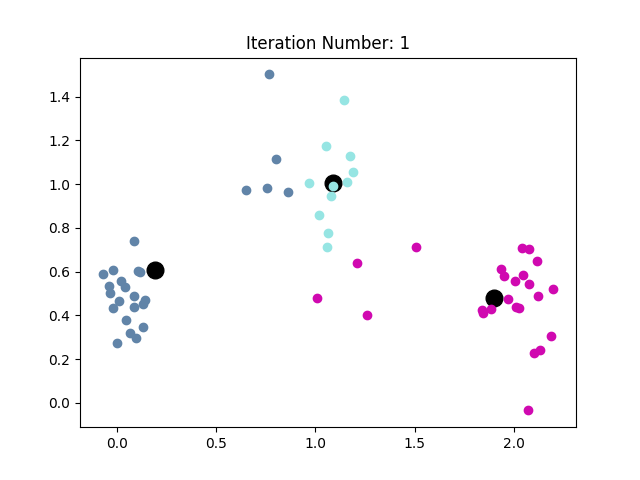
\includegraphics[scale=0.4]{means_1.png} 
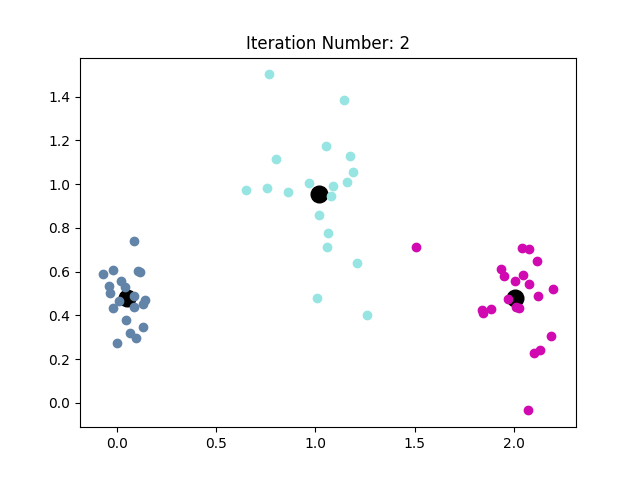
\includegraphics[scale=0.4]{means_2.png} \newline
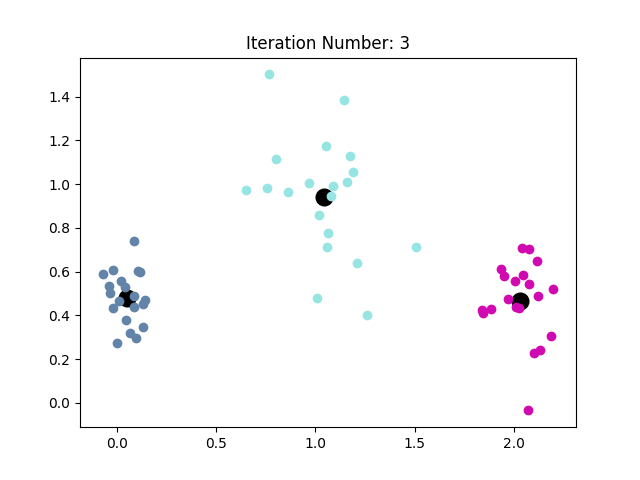
\includegraphics[scale=0.4]{means_3.png}
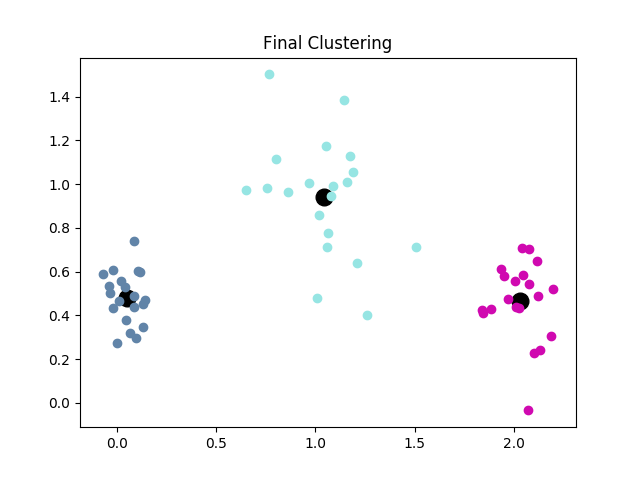
\includegraphics[scale=0.4]{means_final.png} 

The cluster centers for each of the above iterations is as follows
\begin{center}
	\scalebox{0.8}{
	\begin{tabular}{c | c | c | c}
		Iteration Number & Cluster Center 1 & Cluster Center 2 & Cluster Center 3 \\
		\hline
		1 & (1.061948,0.775711) & (1.210252,0.638547) & (0.649507,0.974770) \\
		\hline
		2 & (1.089668,1.004243) & (1.900104,0.480904) & (0.192982,0.606416) \\
		\hline		
		3 & (1.016055,0.952888) & (2.005941,0.477239) & (0.049180,0.481094) \\
		\hline		
		Final & (1.040635,0.940960) & (2.030856,0.465384) & (0.049180,0.481094) \\
	
	\end{tabular}}
\end{center}

\item 
The graphs for random initialization with kMedoids looks like the following: \newline
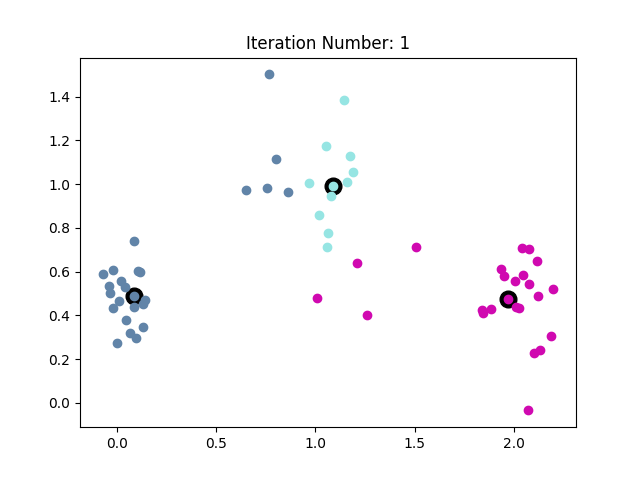
\includegraphics[scale=0.4]{medoid_1.png}
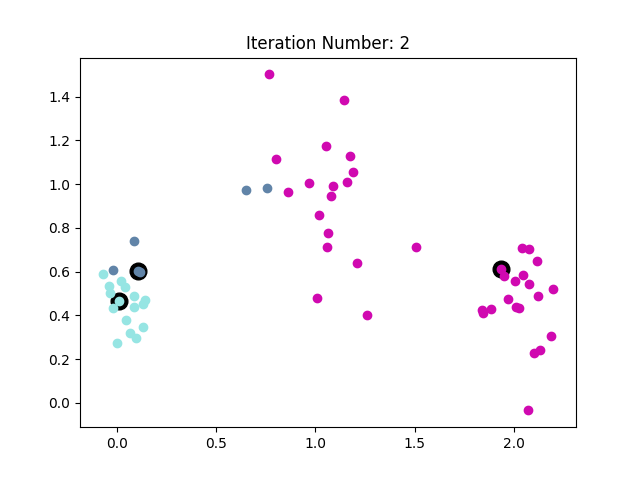
\includegraphics[scale=0.4]{medoid_2.png} \newline
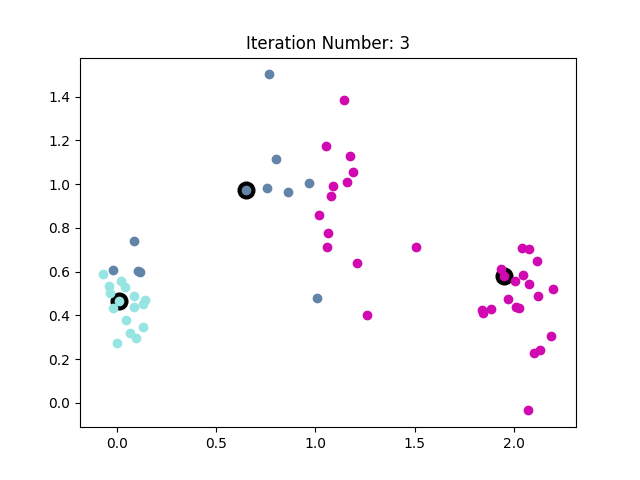
\includegraphics[scale=0.4]{medoid_3.png}
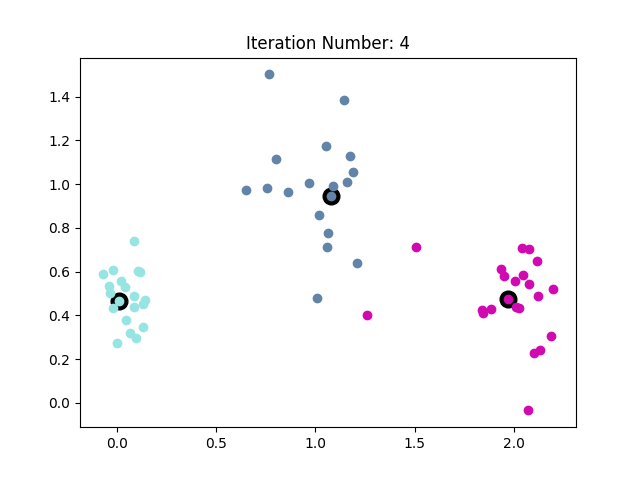
\includegraphics[scale=0.4]{medoid_4.png} \newline
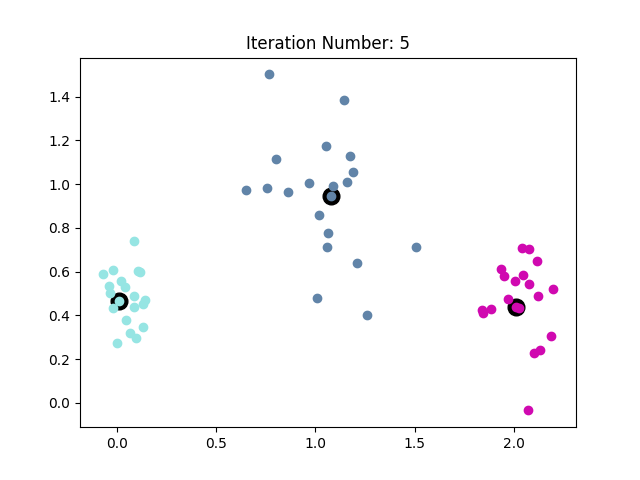
\includegraphics[scale=0.4]{medoid_5.png}
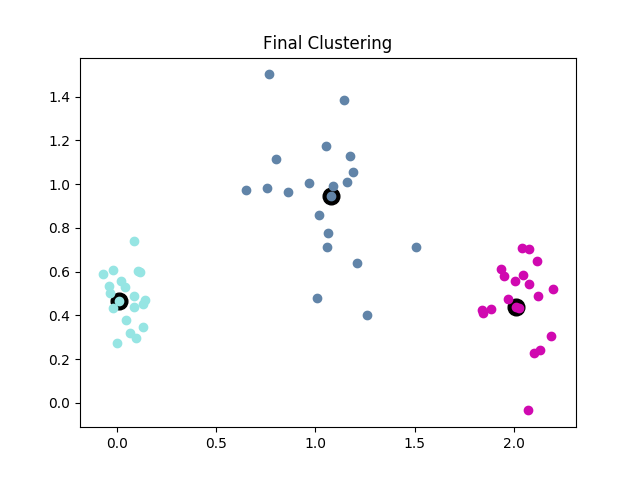
\includegraphics[scale=0.4]{medoid_final.png} \newline
The cluster centers for each of the above iterations is as follows
\begin{center}
	\scalebox{0.8}{
	\begin{tabular}{c | c | c | c}
		Iteration Number & Cluster Center 1 & Cluster Center 2 & Cluster Center 3 \\
		\hline
		1 & (-0.033408,0.500212) & (1.157995,1.009878) & (0.084167,0.739096) \\
		\hline		
		2 & (0.012471,0.467721) & (1.507651,0.714342) & (0.104758,0.604594) \\
		\hline		
		3 & (0.012471,0.467721) & (1.932385,0.612375) & (0.104758,0.604594) \\
		\hline		
		4 & (0.012471,0.467721) & (1.948285,0.579243) & (0.649507,0.974770) \\
		\hline		
		5 & (0.012471,0.467721) & (1.969410,0.472674) & (1.076992,0.947875) \\
		\hline		
		Final & (0.012471,0.467721) & (2.011976,0.440005) & (1.076992,0.947875) \\
	\end{tabular}}
\end{center}
\end{enumerate}
\end{document}
